\documentclass[12pt]{exam}
\usepackage{epsfig}
\usepackage[usenames,dvipsnames,svgnames,table]{xcolor}
\usepackage{listings}
\usepackage{color}
\usepackage{float}
\usepackage{bookmark}
\usepackage{paralist}

% Must be last
\usepackage{hyperref}

\hypersetup{
    colorlinks=true,
    linkcolor=blue,
    filecolor=magenta,
    urlcolor=blue,
}

\newcommand{\note}[1]{\marginpar{\LARGE $\spadesuit$}
      $\spadesuit$ {\bf #1} $\spadesuit$}
      
\lstdefinestyle{error}{
  emptylines=1,
  breaklines=true,
  basicstyle=\ttfamily\color{red}
}

\lstdefinestyle{command}{
  emptylines=1,
  breaklines=true,
  basicstyle=\ttfamily\color{black}
}


\pagestyle{headandfoot}
\firstpageheader{}{}{}
\runningheader{CPSC 314}{Assignment 2}{Due Oct 22, 2021}
\setlength{\parindent}{0pt}
\begin{document}

\title{CPSC 314\\
  Assignment 2: Transformations}
\date{Due 11:59PM, October 22, 2021}

\maketitle 

\section{Introduction}

In this assignment you will utilize your knowledge of transformations to make things move.
We will take a look at how to build and animate object hierarchies. As for our subject,
we continue on from Assignment 1 with our armadillo.

\subsection{Getting the Code}
Assignment code is hosted on the UBC Students GitHub. To retrieve it
onto your local machine navigate to the folder on your machine where you intend to keep your
assignment code, and run the following command from the terminal or command line:

\medskip
{\tt git clone https://github.students.cs.ubc.ca/cpsc314-2021w-t1/a2-release.git}

\subsection{Template}
\begin{itemize}
\item The file {\tt A2.html} is the launcher of the assignment. Open
  it in your preferred browser to run the assigment, to get started.
\item The file {\tt A2.js} contains the JavaScript code used to set up the scene and the rendering environment. You will need to make minor changes in it to answer the questions.
\item The folder {\tt glsl} contains the vertex and fragment shaders for the armadillo and sphere geometry. This is where you will do most of your coding.
\item The folder {\tt js} contains the required JavaScript libraries. You do not need to change anything here.
\item The folder {\tt obj} contains the geometric models loaded in the scene.
\item The folder {\tt images} contains the texture images used.
\end{itemize}

\subsection{Execution}
As mentioned above, the assignment can be run by opening the file {\tt
  A2.html} in any modern browser. However, most browsers will prevent
pages from accessing local files on your computer. If you simply open
{\tt A2.html}, you may get a black screen and an error message on the
console similar to this:
\begin{lstlisting}[style = error]
    XMLHttpRequest cannot load... Cross origin requests are only supported for protocol schemes: http, data, https.
\end{lstlisting}

Please see this web page for options on how to run things locally:
\begin{quotation}
    {\footnotesize \url{https://threejs.org/docs/\#manual/en/introduction/How-to-run-things-locally}}
\end{quotation}

We highly recommend that you run a local server, instead of changing browser security settings.

\begin{enumerate}
    \item Follow the link \url{https://nodejs.org/en/} to download and install Node.js, which
        comes packaged with npm.
    \item Open the link \url{https://www.npmjs.com/package/http-server} and follow the
        instructions to download and install a local command-line http server.
    \item Go to the command-line or terminal and run {\tt http-server [path]}
        where [path] is the path to the assignment folder.
    \item Open your preferred browser and copy and paste the URL of the
        local server specified by the http-server on your command-line.
\end{enumerate}

\newpage

\section{Work to be done (100 pts)}

First, ensure that you can run the template code in your browser. See
the instructions above. Study the template to get a sense of how it
works. The script {\tt js/setup.js} creates the basic scene with the floor, and provides a utility function for loading 3D models. The initial configuration should look as it does in the figure below. For all parts,
it will be helpful to look at Three.JS's documentation \url{https://threejs.org/docs/}, and lecture materials on scene graphs and hierarchies.

\begin{figure}[H]
    \centering
    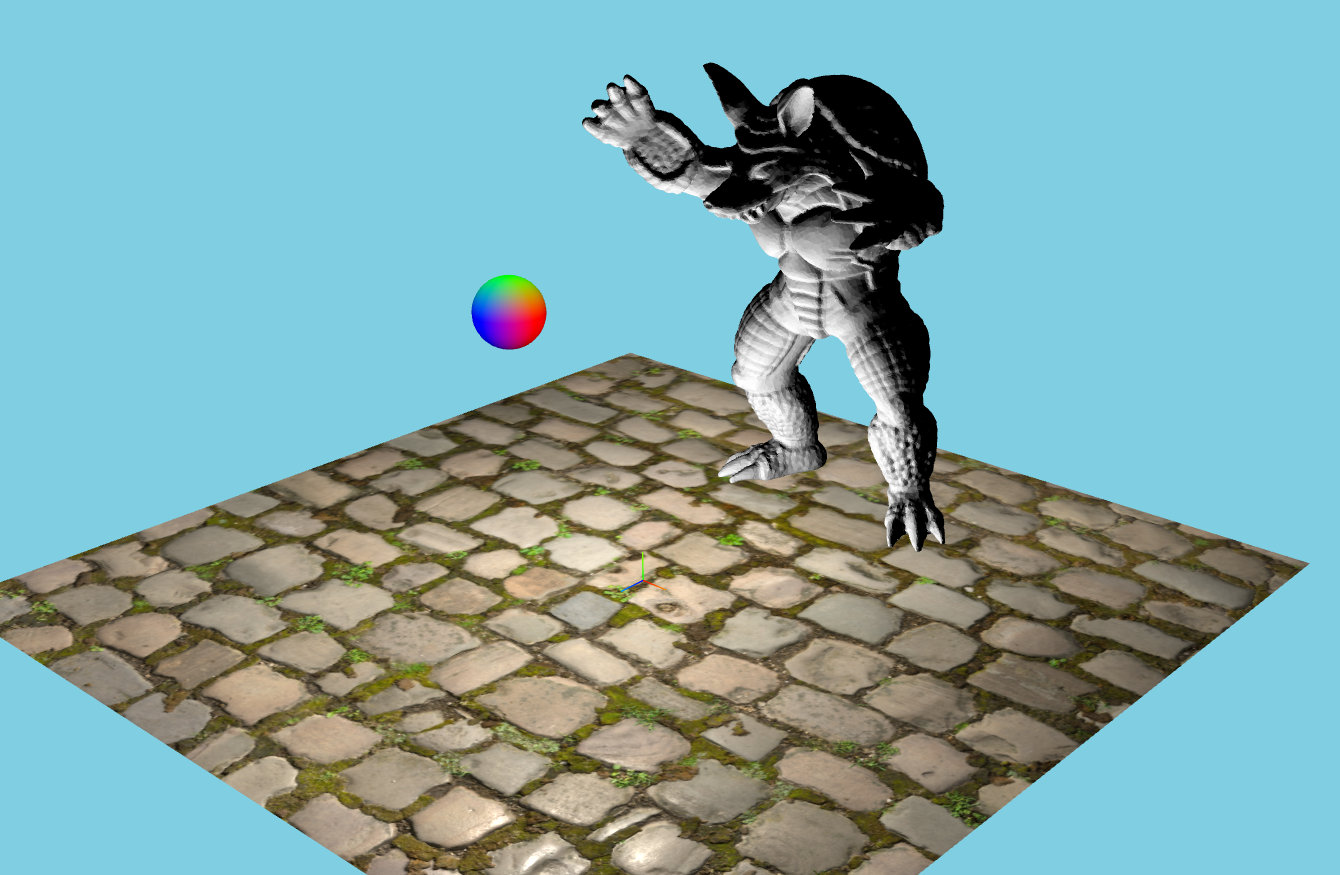
\includegraphics[width=0.3\textwidth]{./init.png}
\end{figure}

{\bf Part 1: Required Elements}

\renewcommand{\labelenumi}{(\alph{enumi})}
\begin{enumerate}

\item {\bf 15 pts} Adding eyes
\label{ref:simpleorb}

For the first part of the assignment you will give the armadillo eyes. In the code you'll see that there are two eyeball meshes provided. Your task is to add them to the scene and ensure  their position is roughly as depicted in the image below. 

  \textit{Hint 1: }This part can be done entirely in {\tt A2.js} 

    \begin{figure}[H]
    \centering
    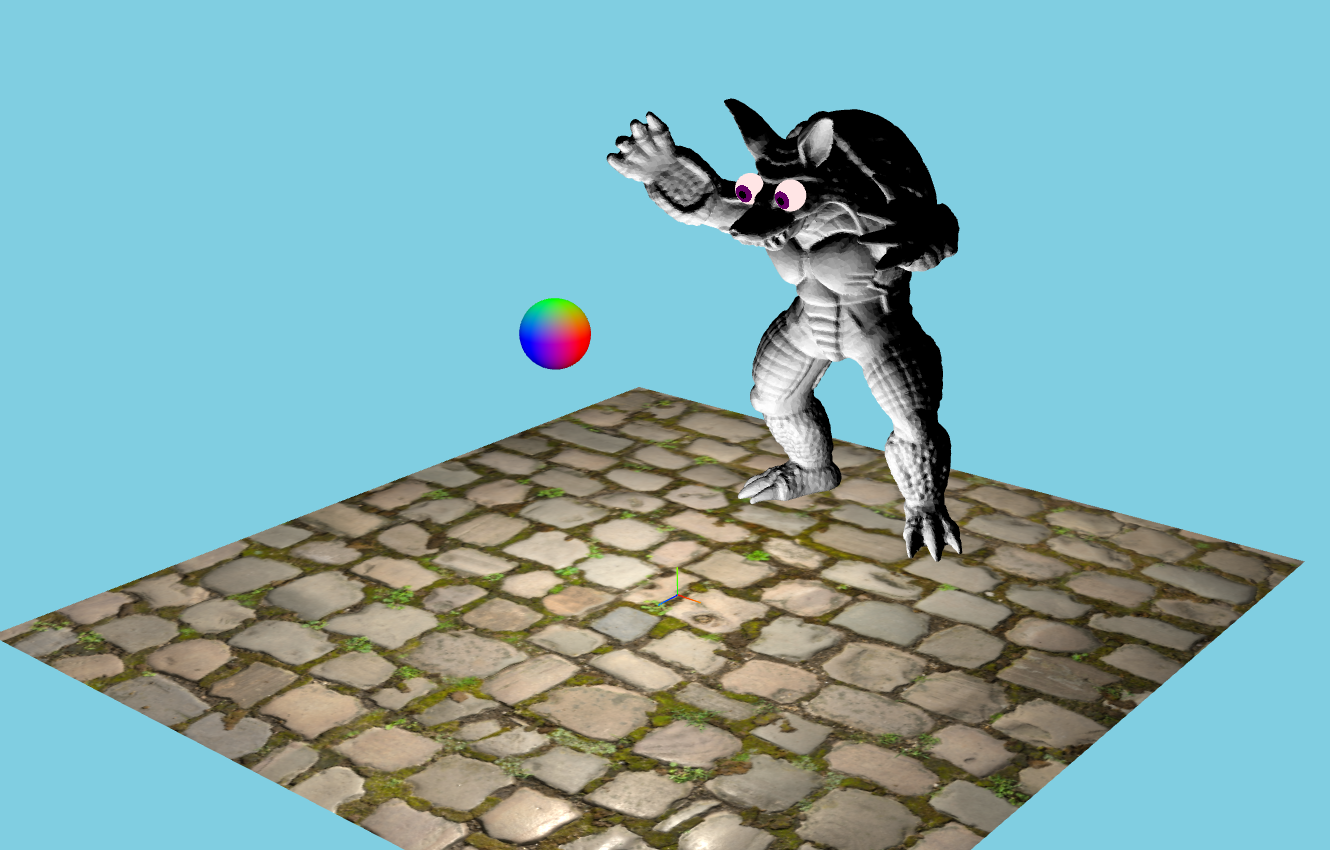
\includegraphics[width=0.3\textwidth]{./qa.png}
    \end{figure}
    
\item {\bf 15 pts} Lasers
\label{ref:simpleorb}

  Now that our armadillo can see, let's make him Superman. You will use the provided cylinder geometry, along with the beam materials, to  make the armadillo shoot lasers out of its eyes at the orb. You should use three.js’ Matrix class and its associated functionality to define the transformation that will achieve the desired effect, then pass that Matrix (as a uniform) into the shaders where it will be applied to the model. 
    \textit{Hint 1: } {\tt THREE.Matrix4} and {\tt THREE.Object3D} have a method called {\tt lookAt} that may be of use. 
    
    \begin{figure}[H]
    \centering
    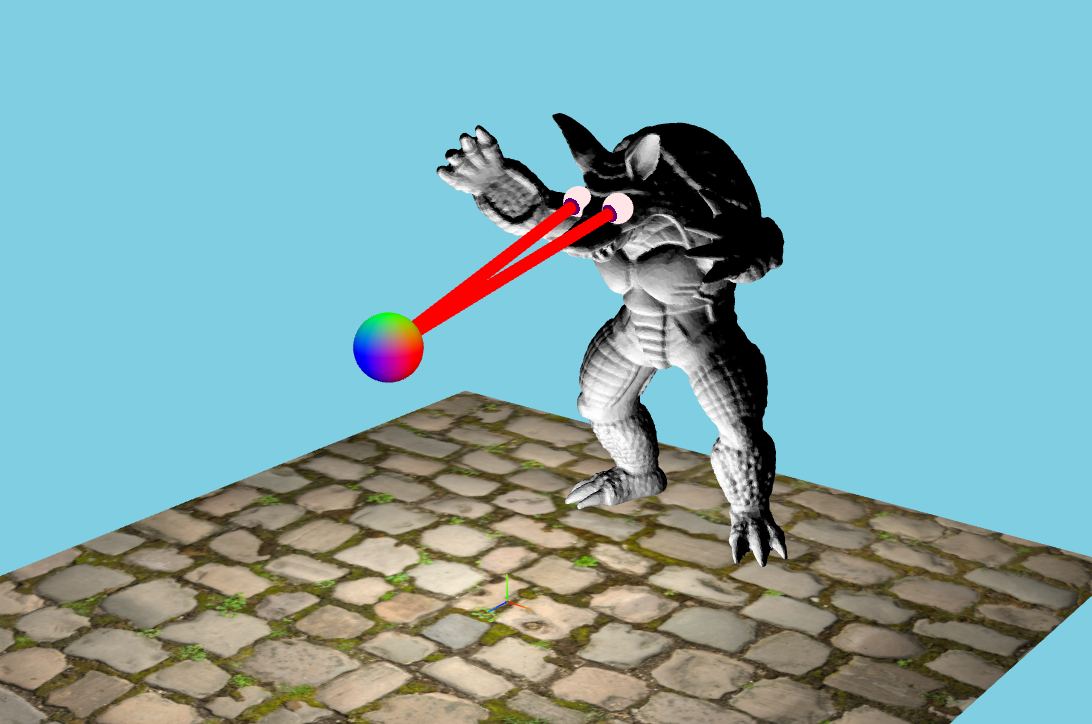
\includegraphics[width=0.3\textwidth]{./qb.png}
    \end{figure}

\item {\bf 35 pts} Tracking.
    The next step is to give our armadillo a moving target and the ability to hit it.  Make the sphere orb in the scene move by responding to keyboard input (WASD can be used for horizontal movement and QE can be used for vertical movement). Add an update function which will adjust the transformation of the lasers so that they are continuously pointing from the eye to the orb. 
    


\item {\bf 35 pts} Orb Deformation

 Add some deformation to the orb by transforming the vertices of the sphere orb. Scale the position of the vertices so that the orb changes sinusoidally with time. You can pass the time as a uniform variable to the shader for the orb. You may come up with and implement any interesting deformation for this section. There are only two requirements: 
\begin{itemize}
\item The size of the orb must change sinusoidally with time.
\item The deformation must be a function on the vertice's position on the sphere.
\end{itemize}
 
This part will require changes in shader code and {\tt A2.js}

The following is an example of a deformation. This deformation changes the orb into a cube sinusoidally over time before changing back to an orb.
 
    \begin{figure}[H]
    \centering
    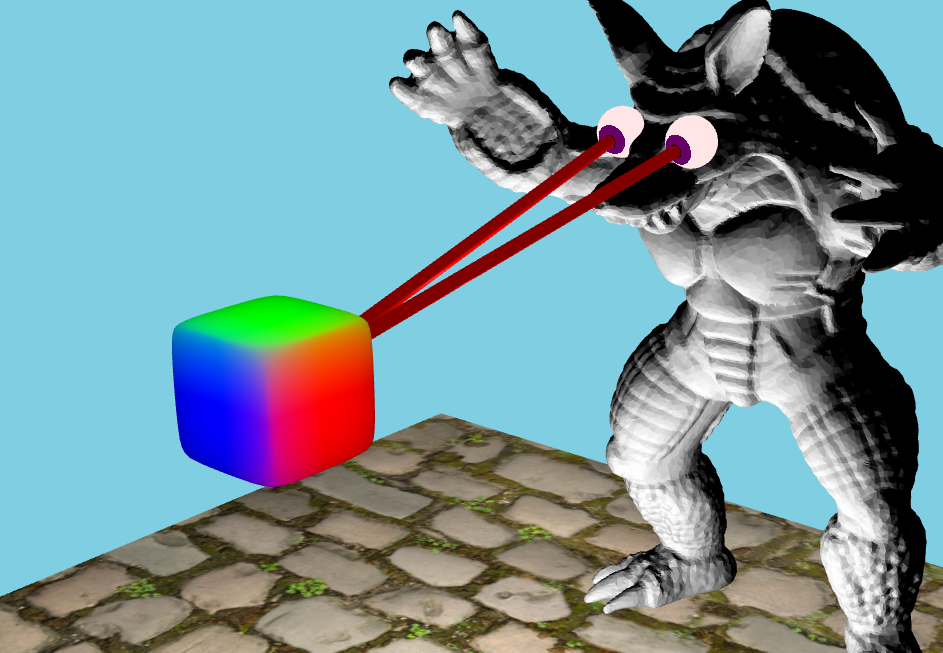
\includegraphics[width=0.3\textwidth]{./last_step.png}
    \end{figure}

  
\end{enumerate}


{\bf Part 2: Creative License (Optional)}

You have many opportunities to unleash your creativity in
computer graphics!  In this \textbf{optional} section, and you are
invited to extend the assignment in fun and creative ways.
We'll highlight some of the best work in class. A small number of
exceptional contributions may be awarded bonus points.
Some possible suggestions might be:
\begin{itemize}
\item Animate other body parts of the armadillo
\item Detect if the armadillo actually reached the ice cream and give him a reward
\item Add other objects to the scene that are animated
\item Make a game out of all this! 
\end{itemize}


\section{Hand-in Instructions}
\subsection{Directory Structure}
Under the root directory of your assignment, create two subdirectories
named ``part1'' and ``part2'', and put all the source files, your
makefile, and everything else required to run each part in the respective
folder. Do not create more sub-directories than the ones already provided. 

You must also write a clear README.txt file that includes your name,
student number, and CWL username, instructions on how to use the
program (keyboard actions, etc.) and any information you would like to
pass on to the marker. Place README.txt under the root directory of your
assigment.

\subsection{Submission Methods}
You can choose one of the two ways to submit your assignment: 
\begin{inparaenum}
  \item running {\tt handin} command on a departmental server, or
  \item submitting through {\tt Web-Handin}.
\end{inparaenum}

\subsubsection{Submit from departmental server}
\begin{enumerate}[1.]
  \item SSH into a departmental server.
  \item Create a directory named ``cs-314'' under your home directory if you have not yet done so.
  \item Create a folder called ``a2'' under {\tt cs-314/}.
  \item Upload everything under the root directory of your assignment to ``a2''.
  \item Run the exact command: {\tt handin cs-314 a2}.
  \item Check if the submission was successful: run {\tt handin -c cs-314 a2}.
\end{enumerate}

\subsubsection{Submit via Web-Handin}
\begin{enumerate}[1.]
  \item Compress everything under the root directory of your assignment into {\tt a2.zip}.
  \item Log into {\tt Web-Handin} with your CWL credentials, by following this link \url{https://my.cs.ubc.ca/docs/hand-in}
  \item Write ``cs-314'' for the course name, ``a2'' for the assignment name.
  \item If you're trying to overwrite a previous submission, check the box "Overwrite previous".
  \item Upload the zip file.
  \item Click "Handin assignment".
  \item Check if the submission was successful: use the {\tt Check submissions} button.
\end{enumerate}

\end{document}
%%% Local Variables:
%%% mode: latex
%%% TeX-master: t
%%% End:
